\documentclass[12pt]{article}
\usepackage[lmargin=.75in,rmargin=.75in,tmargin=.5in,bmargin=1in]{geometry}
\usepackage{amsmath}
\usepackage{amssymb}
\usepackage{amsfonts}
\usepackage{mathrsfs}
\usepackage{theorem}


\usepackage{caption}
\usepackage{subcaption}

\usepackage{graphicx}
\graphicspath{ {images/} }
\usepackage{float}


\newtheorem{theorem}{\bf Theorem}[section]
\newtheorem{lemma}[theorem]{Lemma}
\newtheorem{proposition}[theorem]{Proposition}
\newtheorem{corollary}[theorem]{Corollary}
\theorembodyfont{\rmfamily}
\newtheorem{definition}[theorem]{Definition}
\newtheorem{example}[theorem]{Example}
\newtheorem{conjecture}[theorem]{Conjecture}
\newtheorem{remark}[theorem]{Remark}

\newenvironment{proof}{{\bf Proof:}}{\hfill$\square$}
%\renewcommand{\theequation}{\thesection.\arabic{equation}}
\renewcommand{\thesection}{\arabic{section}}
\renewcommand{\thesubsection}{(\alph{subsection})}


\renewcommand{\thesection}{\thechapter .\arabic{section}}
%\newtheorem{theorem}{\bf Theorem}[section]
%\newtheorem{lemma}[theorem]{\bf Lemma}
%\newtheorem{proposition}[theorem]{\bf Proposition}
%\newtheorem{example}[theorem]{\bf Example}
%\newtheorem{definition}[theorem]{\bf Definition}
%\newtheorem{remark}[theorem]{\bf Remark}
%\newtheorem{corollary}[theorem]{\bf Corollary}
%\numberwithin{equation}{chapter}

%\renewcommand{\thesection}{\thechapter .\arabic{section}}

\newcommand{\numbering}[1]{\refstepcounter{theorem}\label{#1}{\noindent \bf\ref{#1}}}

\newcommand{\Adb}{\mbox{$\mathbb{A}$}}
\newcommand{\Bdb}{\mbox{$\mathbb{B}$}}
\newcommand{\Cdb}{\mbox{$\mathbb{C}$}}
\newcommand{\Ddb}{\mbox{$\mathbb{D}$}}
\newcommand{\Edb}{\mbox{$\mathbb{E}$}}
\newcommand{\Fdb}{\mbox{$\mathbb{F}$}}
\newcommand{\Gdb}{\mbox{$\mathbb{G}$}}
\newcommand{\Hdb}{\mbox{$\mathbb{H}$}}
\newcommand{\Idb}{\mbox{$\mathbb{I}$}}
\newcommand{\Jdb}{\mbox{$\mathbb{J}$}}
\newcommand{\Kdb}{\mbox{$\mathbb{K}$}}
\newcommand{\Ldb}{\mbox{$\mathbb{L}$}}
\newcommand{\Mdb}{\mbox{$\mathbb{M}$}}
\newcommand{\Ndb}{\mbox{$\mathbb{N}$}}
\newcommand{\Odb}{\mbox{$\mathbb{O}$}}
\newcommand{\Pdb}{\mbox{$\mathbb{P}$}}
\newcommand{\Qdb}{\mbox{$\mathbb{Q}$}}
\newcommand{\Rdb}{\mbox{$\mathbb{R}$}}
\newcommand{\Sdb}{\mbox{$\mathbb{S}$}}
\newcommand{\Tdb}{\mbox{$\mathbb{T}$}}
\newcommand{\Udb}{\mbox{$\mathbb{U}$}}
\newcommand{\Vdb}{\mbox{$\mathbb{V}$}}
\newcommand{\Wdb}{\mbox{$\mathbb{W}$}}
\newcommand{\Xdb}{\mbox{$\mathbb{X}$}}
\newcommand{\Ydb}{\mbox{$\mathbb{Y}$}}
\newcommand{\Zdb}{\mbox{$\mathbb{Z}$}}

\newcommand{\A}{\mbox{$\mathscr{A}$}}
%\newcommand{\A}{\mbox{${\mathcal A}$}}
\newcommand{\B}{\mbox{${\mathcal B}$}}
\newcommand{\C}{\mbox{${\mathcal C}$}}
\newcommand{\D}{\mbox{${\mathcal D}$}}
\newcommand{\E}{\mbox{${\mathcal E}$}}
\newcommand{\F}{\mbox{${\mathcal F}$}}
\newcommand{\G}{\mbox{${\mathcal G}$}}
\renewcommand{\H}{\mbox{${\mathcal H}$}}
\newcommand{\I}{\mbox{${\mathcal I}$}}
\newcommand{\J}{\mbox{${\mathcal J}$}}
\newcommand{\K}{\mbox{${\mathcal K}$}}
\newcommand{\Ll}{\mbox{${\mathcal L}$}}
\newcommand{\Mc}{\mbox{${\mathcal M}$}}
\newcommand{\N}{\mbox{${\mathcal N}$}}
\renewcommand{\O}{\mbox{${\mathcal O}$}}
\renewcommand{\P}{\mbox{${\mathcal P}$}}
\newcommand{\Q}{\mbox{${\mathcal Q}$}}
\newcommand{\R}{\mbox{${\mathcal R}$}}
\renewcommand{\S}{\mbox{${\mathcal S}$}}
 \newcommand{\T}{\mbox{${\mathcal T}$}}
 \newcommand{\U}{\mbox{${\mathcal U}$}}
\newcommand{\V}{\mbox{${\mathcal V}$}}
\newcommand{\W}{\mbox{${\mathcal W}$}}
\newcommand{\X}{\mbox{${\mathcal X}$}}
\newcommand{\Y}{\mbox{${\mathcal Y}$}}
\newcommand{\Z}{\mbox{${\mathcal Z}$}}


\begin{document}


\title{\Large Calculus I Question}
\author{SHANG-HUAN CHIU}
\maketitle

Question:
\begin{figure}[H]
       \centering       
               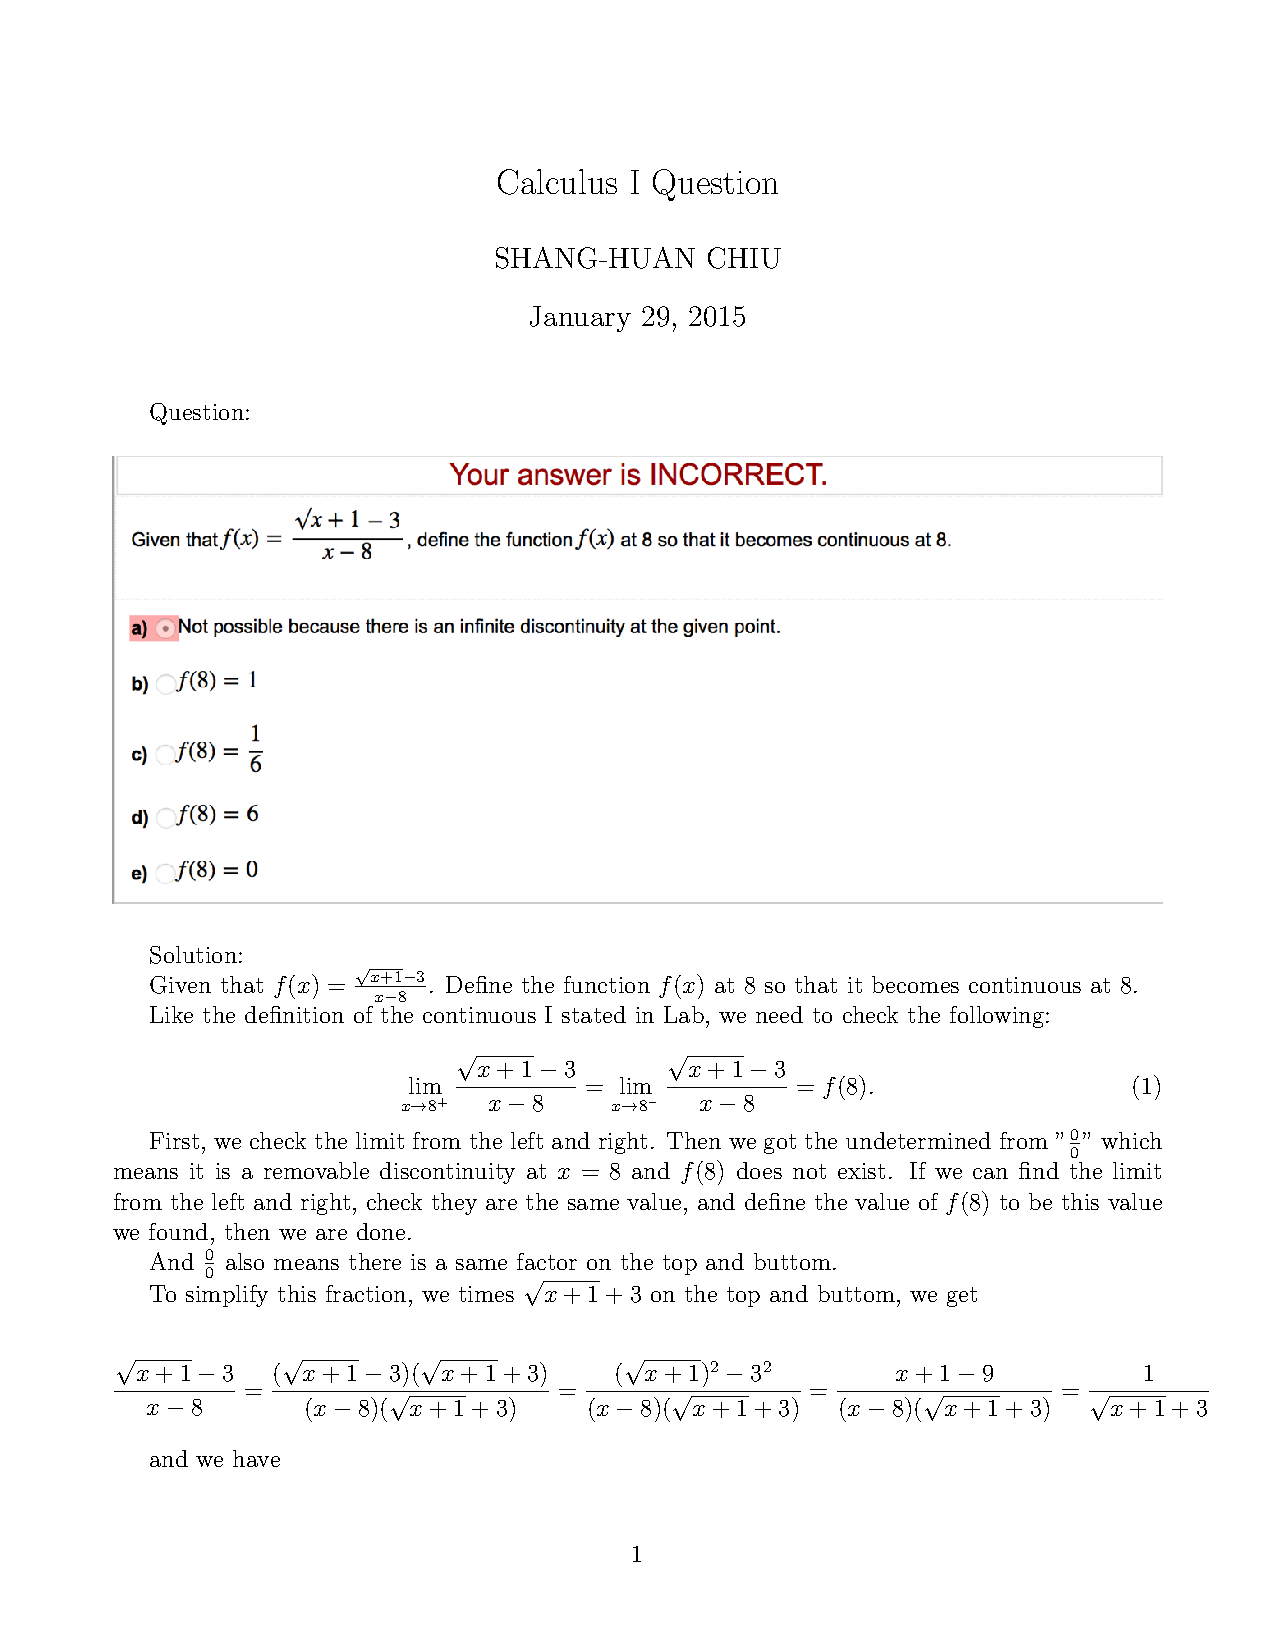
\includegraphics[width=\textwidth]{1431_Question_1}
\end{figure}
Solution:

Given that $f(x)=\frac{\sqrt{x+1}-3}{x-8}$. Define the function $f(x)$ at $8$ so that it becomes continuous at $8$.

Like the definition of the continuous I stated in Lab, we need to check the following:

\begin{equation}\label{def}
\lim_{x \to 8^+}\frac{\sqrt{x+1}-3}{x-8}=\lim_{x \to 8^-}\frac{\sqrt{x+1}-3}{x-8}=f(8).
\end{equation}

First, we check the limit from the left and right. Then we got the undetermined from "$\frac{0}{0}$"
which means it is a removable discontinuity at $x=8$ and $f(8)$ does not exist.
If we can find the limit from the left and right, check they are the same value, and
define the value of $f(8)$ to be this value we found, then we are done.

And $\frac{0}{0}$ also means there is a same factor on the top and buttom. 

To simplify this fraction, we times $\sqrt{x+1}+3$ on the top and buttom, we get

$$\frac{\sqrt{x+1}-3}{x-8}=\frac{(\sqrt{x+1}-3)(\sqrt{x+1}+3)}{(x-8)(\sqrt{x+1}+3)}=
\frac{(\sqrt{x+1})^2 -3^2}{(x-8)(\sqrt{x+1}+3)}=\frac{x+1-9}{(x-8)(\sqrt{x+1}+3)}=\frac{1}{\sqrt{x+1}+3}$$

and we have 

$$\lim_{x \to 8^+}\frac{\sqrt{x+1}-3}{x-8}=\lim_{x \to 8^-}\frac{\sqrt{x+1}-3}{x-8}=\frac{1}{6}.$$

Thus, if we redefine $f(8)=\frac{1}{6}$ which is satified the definition $\eqref{def}$ then
we can say this new $f$ is continuous at $x=8$.





































\end{document}